\chapter{Background and state of the art}
\label{SOTA}

\lettrine[lines=4]{T}{his} chapter discusses the state-of-the-art in the areas of \Wasm and Software Diversification. 
In \autoref{sota:wasm} we discuss \Wasm, focusing on its design and security model.
Besides, we discuss the current state-of-the-art in the area of \Wasm program analysis.
In \autoref{sota:sw} we discuss related works in the area of Software Diversification.
Moreover, we delve into the open challenges regarding the diversification of \Wasm programs.

\msection{\Wasm}
\label{sota:wasm}
%% For the intro
 % In 2014, Alon Zakai and colleagues proposed Emscripten \cite{emscripten}. 
% Emscripten used a strict subset of JavaScript, asm.js, to allow low-level code such as C to be compiled to JavaScript. 
% Asm.js was faster than JavaScript because it limited the language features to those that can be optimized in the LLVM pipeline. 
% Notably, Asm.js demonstrated that client-code could be improved with the right language design and standardization.
% Wasm marked the breaking point of several failed attempts of porting code but JavaScript to the web browser \cite{javaapplet,activex,silverlight}.
% Previous alternatives largely failed to gain traction, primarily due to security concerns and a lack of consensus among browser vendors.
% The announcement of \wasm\ marked the first step into the standardization of bytecode in the web environment. 

% History
The W3C publicly announced the \Wasm(Wasm) language in 2017 as the four scripting language supported in all major web browser vendors.
\wasm\ is a binary instruction format for a stack-based virtual machine and was officially consolidated by the work of Haas \etal \cite{Haas_2017} in 2017 and extended by Rossberg \etal in 2018 \cite{10.1145/3282510}. 
It is designed to be fast, portable, self-contained and secure, and it promises to outperform JavaScript execution. 
Since 2017, the adoption of \wasm\ keeps growing. 
For example; Adobe, announced a full online version of Photoshop\footnote{\url{https://twitter.com/Adobe/status/1453034805004685313?s=20&t=Zf1N7-WmzecA0K4V8R69lw}} written in WebAssembly;  game companies moved their development from JavaScript to Wasm like is the case of a full Minecraft version\footnote{\url{https://satoshinm.github.io/NetCraft/}}. 

Moreover, WebAssembly has been evolving outside web browsers since its first announcement.
Some works demonstrated that using WebAssembly as an intermediate layer is better in terms of startup and memory usage than containerization and virtualization \cite{pMendkiServerless, 1244493Jacobsson}. 
Consequently, in 2019, the Bytecodealliance proposed WebAssembly System Interface (WASI) \cite{WASI}. 
WASI pioneered the execution of \wasm\ with a POSIX system interface protocol, making it possible to execute Wasm closer to the underlying operating system. 
Therefore, it standardizes the adoption of \wasm\ in heterogeneous platforms \cite{bryant2020webassembly}, making it suitable for standalone and backend execution scenarios \cite{9640153, wen2020wasmachine}.

% How to generate
%\msubsection{\Wasm's generation and binary format}
%\todo{Replace by Rust example}
%\todo{Annotate the Wasm code with the sections offset and length}
%\todo{Instantiate each one of the previously mentioned concepts}
%\todo{Improve some metadata, size of the code, etc}
%\todo{FIX: linerefs}

\msubsection{From source code to \Wasm}

\Wasm programs are compiled from source languages like C/C++, Rust, or Go, which means that it can benefit from the optimizations of the source language compiler.
The resulting \wasm program is like a traditional shared library, containing instruction codes, symbols, and exported functions. 
A host environment is in charge of complementing the Wasm program, such as providing external functions required for execution within the host engine. 
For instance, functions for interacting with an HTML page's DOM are imported into the Wasm binary when invoked from JavaScript code in the browser. 


In \autoref{CExample1} and \autoref{WASMExample}, we illustrate a C program and its corresponding Wasm binary. 
The C function includes heap allocation, external function usage, and a function definition featuring a loop, conditional branching, function calls, and memory accesses. 
The Wasm code in \autoref{WASMExample} displays the textual format of the generated Wasm (Wat)\footnote{The WAT text format is mostly for human readability and for low-level manual modification.}.



\begin{minipage}[hbtp]{0.9\textwidth}
    \begin{minipage}[t]{1.0\linewidth}
        \lstset{language=C,caption={Example C program which includes heap allocation, external function usage, and a function definition featuring a loop, conditional branching, function calls, and memory accesses.  },
        label=CExample1,
        breaklines=true, 
        basicstyle=\small\ttfamily,
        captionpos=b,
        frame=b,
        numbers=none,
        postbreak=\mbox{\textcolor{red}{$\hookrightarrow$}\space},
        escapeinside={(*@}{@*)}
        }
    \input{sota/code/code.c}
    \end{minipage}
\end{minipage}



\begin{minipage}[hbtp]{0.9\textwidth}
  

    \begin{minipage}[t]{1.0\linewidth}
    \lstset{
        language=WAT,
        caption={ Refer to \autoref{CExample1} for the Rust code example. This example showcases the translation from Rust to \wasm. For clarity, we have marked elements and portions of the \Wasm binary as comments.},
        style=WATStyle,
        breaklines=true, 
        %stepnumber=0,
        captionpos=b,
        frame=b,
        escapeinside={(*@}{@*)},
        numbers=none,
        postbreak=\mbox{\textcolor{red}{$\hookrightarrow$}\space},
        label=WASMExample}
    %
    \input{sota/code2/fibo.shortest.wat}
    %\end{lstlisting}
    \end{minipage}
\end{minipage}

\msubsection{\Wasm's binary format}
\label{background:wasm:binary}

The Wasm binary format is close to machine code and already optimized, being a consecutive collection of sections.
In \autoref{background:wasm:fig:section} we show the binary format of a Wasm section.
A Wasm section starts with a 1-byte section ID, followed by a 4-byte section size, and concludes with the section content, which precisely matches the size indicated earlier.
A \wasm binary contains sections of 13 types, each with a specific semantic role and placement within the module. 
Each section is optional, where an omitted section is considered empty.
In the following, we summarize each one of the 13 types of \wasm sections, providing their name, ID, and purpose. 
In addition, some sections are annotated as comments in the Wasm code in \autoref{WASMExample}.
    
\begin{figure}[h]
    \centering
    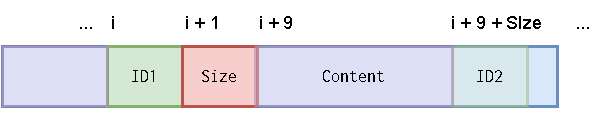
\includegraphics[width=0.5\linewidth]{figures/section.pdf}
    \caption{Memory byte representation of a \Wasm binary section, starting with a 1-byte section ID, followed by an 8-byte section size, and finally the section content.}
    \label{background:wasm:fig:section}
\end{figure}

\wrule{Custom Section (\texttt{00})}: Comprises two parts: the section name and arbitrary content. Primarily used for storing metadata, such as the compiler used to generate the binary (see lines 9 and 48 of \autoref{WASMExample}). This type of section has no order constraints with other sections and is optional. Compilers usually skip this section when consuming a \Wasm binary. 

\wrule{Type Section (\texttt{01})}: Contains the function signatures for functions declared or defined within the binary (see lines 3 to 6 in \autoref{WASMExample}). Functions may share the same function signature. This section must occur only once in a binary. It can be empty. 

\wrule{Import Section (\texttt{02})}: Lists elements imported from the host, including functions, memories, globals, and tables (see line 8 in \autoref{WASMExample}). This section is needed to enable code and data sharing with the host engine and other modules. It must occur only once in a binary. It can be empty.

\wrule{Function Section (\texttt{03})}: Details functions defined within the binary. It essentially maps Type section entries to Code section entries. The text format already maps the function index to its name, as shown in lines 12 to 38 of \autoref{WASMExample}. This section must occur only once in a binary and, it can be empty. 

\wrule{Table Section (\texttt{04})}: Groups functions with identical signatures to control indirect calls. It must occur only once in a binary. It can be empty. The example code in \autoref{WASMExample} does not include a Table Section.

\wrule{Memory Section (\texttt{05})}: Specifies the number and initial size of unmanaged linear memories (see line 40 in \autoref{WASMExample}). It must occur only once in a binary. It can be empty. 

\wrule{Global Section (\texttt{06})}: Defines global variables as managed memory for use and sharing between functions in the \Wasm binary (see line 42 of \autoref{WASMExample}). It must occur only once in a binary. It can be empty.

\wrule{Export Section (\texttt{07})}: Declares elements like functions, globals, memories, and tables for host engine access (see lines 44 and 45 of \autoref{WASMExample}). It must occur only once in a binary. It can be empty.

\wrule{Start Section (\texttt{08})}:  Designates a function to be called upon binary readiness, initializing the \Wasm program state before executing any exported functions. It must occur only once in a binary. It can be empty. The example code in \autoref{WASMExample} does not include a Start Section, i.e. there is no function to call when the binary is initialized.

\wrule{Element Section (\texttt{09})}: Contains elements to initialize the binary tables. It must occur only once in a binary. It can be empty. The example code in \autoref{WASMExample} does not include an Element Section.

\wrule{Code Section (\texttt{10})}: Contains the body of functions defined in the Function section. Each entry consists of local variables used and a list of instructions (see lines 12 to 38 in \autoref{WASMExample}). It must occur only once in a binary. It can be empty.

\wrule{Data Section (\texttt{11})}: Holds data for initializing unmanaged linear memory. Each entry specifies the offset and data to be placed in memory (see line 47 in \autoref{WASMExample}). It must occur only once in a binary. It can be empty.

\wrule{Data Count Section (\texttt{12})}: Primarily used for validating the Data Section. If the segment count in the Data Section mismatches the Data Count, the binary is considered malformed. The example code in \autoref{WASMExample} does not include a Data Count Section.
It must occur only once in a binary. It can be empty.


\vspace{2mm}
Due to its organization into a contiguous array of sections, a \wasm binary can be processed efficiently. 
For example, this structure allows compilers to speed up the compilation process through parallel parsing or just by ignoring \emph{Custom Sections}.
Additionally, the use of the LEB128\toolcite{https://en.wikipedia.org/wiki/LEB128} encoding of instructions of the \emph{Code Section} further compacts the binary. 
As a result, Wasm binaries are not only fast to validate and compile but also quick to transmit over a network.

\msubsection{\Wasm's runtime structure}
\label{background:wasm:execution}


The \Wasm runtime structure is described in the WebAssembly specification by enunciating 10 key components: the Store, Module Instances,  Table Instances, Export Instances, Import Instances, the Execution Stack, Memory Instances, Global Instances, Function Instances and Locals.  
These components are particularly significant in maintaining the state of a WebAssembly program during its execution. 
In the following, we provide a brief description of each runtime component.
Notice that, the runtime structure is an abstraction that serves to validate the execution of a \wasm binary.

\wrule{Store}: The WebAssembly store represents the global state and is a collection of instances of functions, tables, memories, and globals. Each of these instances is uniquely identified by an address, which is usually represented as an i32 integer.


\wrule{Module Instances}: A module instance is a runtime representation of a loaded and initialized WebAssembly module (the binary file described in \autoref{background:wasm:binary}). 
It contains the runtime representation of all the definitions within a module, including functions, tables, memories, and globals, as well as the module's exports and imports.


\wrule{Table instances}: A table instance is a vector of \emph{function instances} with the same signature. 
They are used to validate and support indirect function calls during runtime.
A table instance can be modified through table instructions from the function bodies.


\wrule{Export Instances}: Export instances represent the functions, tables, elements, globals or memories that are exported by a \wasm binary to the host environment. 

\wrule{Import Instances}: Import instances represent the functions, tables, elements, globals or memories that are imported into a module from the host environment. 

\wrule{The Execution Stack} holds typed values, labels and control frames, with labels handling block instructions, loops, and function calls.
Values inside the stack can be of the only static types allowed in Wasm 1.0, \texttt{i32} for 32 bits signed integer, \texttt{i64} for 64 bits signed integer, \texttt{f32} for 32 bits float and \texttt{f64} for 64 bits float.
Therefore, abstract types, such as classes, objects, and arrays, are not natively supported. 
Instead, during compilation, such types are transformed into primitive types and stored in the linear memory.

\wrule{Memory Instances} represent the unmanaged linear memory of a WebAssembly program, consisting of a contiguous array of bytes.
Memory instances are accessed with \texttt{i32} pointers (integer of 32 bits). 
Memory instances are usually bound in browser engines to 4Gb of size, and it is only shareable between the process that instantiates the \Wasm module and the binary itself.

\wrule{Global Instances}: A global instance is a global variable with a value and a mutability flag, indicating whether the global can be modified or is immutable.
Global variables are part of the managed data, i.e., their allocation and memory placement are managed by the host engine.
Global variables are only accessible by their declaration index, and it is not possible to dynamically address them. 


\wrule{Locals}: Locals are mutable variables that are local to a specific function instance, i.e. locals are only accessible through their index related to the executing function instance. As globals, locals are part of the managed data.

\wrule{Function Instances}: are closures over the runtime module instance.
A function instance groups locals and a function body.
Locals are typed variables that are local to a specific function invocation as previously discussed.
The function body is a sequence of instructions that are executed when the function is called.
Each instruction either reads from the stack, writes to the stack, or modifies the control flow of the function.
Recalling the example \wasm binary previously showed, 
% Functions
the local variable declarations and typed instructions that are evaluated using the stack can be appreciated between Line 7 and Line 32 in \autoref{WASMExample}. 
Each instruction reads its operands from the stack and pushes back the result. 
In the case of \autoref{WASMExample}, the result value of the main function is the calculation of the last instruction, \texttt{i32.add}. 
As the listing also shows, instructions are annotated with a numeric type.


\begin{definition}\label{managed_unmanaged}
    Along with this dissertation, as the work of Lehmann \etal \cite{usenixWasm2020}, we refer to managed and unmanaged data to differentiate between the data that is managed by the host engine and the data that is managed by the \Wasm program respectively. 
\end{definition}


\msubsection{\Wasm's control flow}

In \Wasm, a defined function instructions are organized into blocks, with the function's starting point serving as the root block. 
Unlike traditional assembly code, control flow structures in Wasm jump between block boundaries rather than arbitrary positions within the code. 
Each block might specify the required stack state before execution and the resulting stack state after its instructions have run. 
This stack state is used to validate the binary during compilation and to ensure that the stack is in a valid state before executing the block's instructions.
Blocks in Wasm are explicit, indicating, where they start and end.
By design, each block cannot reference or execute code from outer blocks.

Control flow within a function is managed through three types of break instructions: unconditional break, conditional break, and table break. 
Importantly, each break instruction is limited to jumping to one of its enclosing blocks.
%Loops in Wasm are specialized blocks that can be restarted using a break instruction. 
Unlike standard blocks, where breaks jump to the end of the block, breaks within a loop block jump to the block's beginning, effectively restarting the loop. 
To illustrate this, \autoref{background:wasm:block} provides an example comparing a standard block and a loop block in a Wasm function.


\begin{minipage}{0.95\linewidth}
   
   \begin{minipage}{0.45\linewidth}
      \lstset{
      language=WAT,
      style=WATStyle,
      breaklines=true, 
      %stepnumber=0,
      escapeinside={(*@}{@*)},
      numbers=none,
      postbreak=\mbox{\space},
      label=BlockExample}

   \begin{lstlisting}    
block
   block
      br 1 (*@\tikzmarkMap{2}{}{8.5}{2}{2cm}@*) ; Jump instructions are annotated with the depth of the block they jump to; 
   end (*@\tikzmarkMap{7}{}{8.5}{0}{2cm}@*)
end (*@\tikzmarkMap{1}{}{8}{3}{2cm}@*)
... (*@\tikzmarkMap{9}{}{8.5}{2}{2cm}@*)
   \end{lstlisting}
   \end{minipage}\hspace{1mm}
   \begin{minipage}{0.44\linewidth}
   \lstset{
      language=WAT,
      style=WATStyle,
      breaklines=true, 
      %stepnumber=0,
      escapeinside={(*@}{@*)},
      numbers=none,
      postbreak=\mbox{\space},
      label=LoopExample}

   \begin{lstlisting}    
loop (*@\tikzmarkMap{6}{}{8.5}{2}{2cm}@*)
   ...
   br 0 (*@\tikzmarkMap{5}{}{8.5}{2}{2cm}@*) ;first-order break;
   ... 
end (*@\tikzmarkMap{3}{}{8.5}{2}{2cm}@*) ; end instructions break the block and jump to next instruction; 
... (*@\tikzmarkMap{4}{}{8.5}{-2}{2cm}@*)
   \end{lstlisting}
   \end{minipage}
   \begin{tikzpicture}[remember picture,overlay]

      %\path (2.west) edge[<-, black] (1.west);
      %\path (3.west) edge[<-,  black] (4.west);
   
      \path (1.west) edge[<-, bend right, black] (2.west);
      %\path (1.west) edge[<-, bend right, gray] (7.west);
      %\path (9.west) edge[<-, bend right, gray] (1.west);
   
      \path (4.west) edge[<-, bend right, gray] (3.west);
      \path (6.west) edge[<-, bend left, black] (5.west);
      %\path (9.east) edge[<-, bend right, black] (4.east);
      %\path (7.east) edge[<-, bend right, black] (8.east);
   
      \end{tikzpicture}
      \centering
      \hrule
      \vspace{2mm}
      \captionof{lstlisting}{Example of breaking a block and a loop in \Wasm.}
      \label{background:wasm:block}
\end{minipage}
% Example


Each break instruction includes the depth of the enclosing block as an operand. 
This depth is used to identify the target block for the break instruction. 
For example, in the left-most part of the previously discussed listing, a break instruction with a depth of 1 would jump past two enclosing blocks.


\msubsection{\Wasm's ecosystem}
\label{background:wasm:ecosystems}

%\todo{Split in two sections. Do a new section on WebAssembly analysis.}
%\todo{Other WebAssembly tools section.}

\Wasm programs are tailored for execution in host environments, most notably web browsers. 
The \Wasm ecosystem is a diverse landscape, featuring a multitude of stakeholders and a comprehensive suite of tools to meet various requirements \cite{Avenger}. 
In this section, we delineate two key categories of tools within this ecosystem: compilers and executors. 
Compilers are responsible for converting source code into \Wasm binaries, while executors handle a range of tasks including validation, optimization, machine code transpilation, and actual execution of these \Wasm binaries. 
Executors are often found in browser clients, among other platform

\wrule{Compilers} transform source code into \Wasm binaries. 
For example, LLVM has offered \Wasm as a backend option since its 7.1.0 release\toolcite{https://github.com/llvm/llvm-project/releases/tag/llvmorg-7.1.0}, supporting a diverse set of frontend languages like C/C++, Rust, Go, and AssemblyScript\footnote{A subset of the TypeScript language}.
Significantly, a study by Hilbig et al. reveals that 70\% of \Wasm binaries are generated using LLVM-based compilers. 
In parallel developments, the KMM framework\toolcite{https://kotlinlang.org/docs/wasm-overview.html} has incorporated \Wasm as a compilation target, and the Javy approach\toolcite{https://github.com/bytecodealliance/javy} focuses on encapsulating JavaScript code within isolated \Wasm binaries. 
This latter is achieved by porting both the engine and the source code into a secure \Wasm environment. 
Similarly, Blazor also enables the compilation of C# code into \Wasm binaries for browser execution\footnote{\url{https://dotnet.microsoft.com/apps/aspnet/web-apps/blazor}}.

From a security standpoint, \Wasm programs are designed without a standard library and are prohibited from direct interactions with the operating system. Instead, the host environment offers a predefined set of functions that can be imported into the \Wasm program. 
It falls upon the compilers to specify which functions from the host environment will be imported by the \Wasm application.

\wrule{Browser} engines like V8\toolcite{https://chromium.googlesource.com/v8/v8.git} and SpiderMonkey\toolcite{https://spidermonkey.dev/} are at the forefront of executing \Wasm binaries in browser clients. 
These engines leverage Just-In-Time (JIT) compilers to convert \Wasm into machine code. 
This translation is typically a straightforward one-to-one mapping, given that \Wasm is already an optimized format closely aligned with machine code, as previously discussed in \autoref{background:wasm:binary}. 
For example, V8 just employs quick, rudimentary optimizations, such as constant folding and dead code removal, to guarantee fast readiness for a \wasm binary to execute \cite{10.1145/3282510}.

\wrule{Standalone engines:} \wasm has expanded beyond browser environments, largely due to the WASI\cite{WASI}. 
It standardizes the interactions between host environments and \Wasm modules through a POSIX-like interface.
\wasm compilers can generate binaries that use WASI.
Standalone engines can then execute these binaries in a variety of environments, including cloud, server, and IoT devices.
For example, standalone engines like WASM3\toolcite{https://github.com/wasm3/wasm3}, Wasmer\toolcite{https://wasmer.io/}, Wasmtime\toolcite{https://github.com/bytecodealliance/wasmtime}, WAVM\toolcite{https://github.com/WAVM/WAVM}, and Sledge\cite{Sledge} have emerged to support \Wasm and WASI. 
In a similar vein, Singh et al.\cite{WARDuino2019} introduced a virtual machine for \Wasm tailored for Arduino-based devices. 
Salim et al.\cite{trufflewasm} proposed TruffleWasm, an implementation of \Wasm hosted on Truffle and GraalVM. 
Additionally, SWAM\toolcite{https://github.com/satabin/swam} stands out as \Wasm interpreter implemented in Scala. 
Finally, WaVe\cite{wave} offers a \Wasm interpreter featuring mechanized verification of the \Wasm-WASI interaction with the underlying operating system.



\msubsection{WebAssembly's binary analysis}
\label{background:wasm:analysis}
As the WebAssembly ecosystem continues to grow, the need for robust tools to ensure its security and reliability has increased. 
To address this, a variety of tools have been developed that employ different strategies to identify vulnerabilities in \Wasm programs. 
In the following we provide a brief overview of the most relevant tools in this space w.r.t static and dynamic analysis, as well as specialized malware detection.

%% PATCH
\vspace{10mm}
\wrule{Static and dynamic analysis:} 
Tools like Wassail\cite{wassail}, SecWasm\cite{secwasm}, Wasmati\cite{wasmati}, and Wasp\cite{Wasp} leverage techniques such as information flow control, code property graphs, control flow analysis, and concolic execution to detect vulnerabilities in \wasm binaries. 
Remarkably, VeriWasm\cite{veriwasm} stands out as a static offline verifier specifically designed for native x86-64 binaries compiled from \Wasm. 
In the dynamic analysis counterpart, tools like TaintAssembly\cite{taintassembly}, Wasabi\cite{wasabi}, and Fuzzm\cite{fuzzm} offer similar functionalities in vulnerability detection. 
Stiévenart and colleagues have introduced a dynamic approach to slice \Wasm programs based on Observational-Based Slicing (ORBS)\cite{slicing, slicing2}. 
Hybrid methods have also gained traction, with tools like CT-Wasm\cite{ctwasm} enabling the verifiably secure implementation of cryptographic algorithms in \Wasm. 
% Finally, Wafl\cite{wafl} extends AFL++ to perform coverage-based fuzzing on \Wasm binaries.


\wrule{Specialized Malware Detection:} Cryptomalware have a wide presence in the web since the first days of \wasm.
The main reason is that mining algorithms using CPUs moved to \wasm for obvious performance reasons \cite{musch2019new}. 
In cryptomalware detection, tools like MineSweeper\cite{Minesweeper}, MinerRay\cite{MinerRay}, and MINOS\cite{MINOS} utilize static analysis through machine learning techniques to detect browser cryptomalwares. 
Conversely, tools like SEISMIC\cite{SEISMIC}, RAPID\cite{RAPID}, and OUTGuard\cite{outguard} seek the same goal with dynamic analysis techniques.
Remarkably, VirusTotal\toolcite{https://www.virustotal.com}, packaging more than 60 commercial antivirus as back-boxes, detects cryptomalware in \wasm binaries.


\msubsection{\Wasm's security}


While \Wasm is engineered to be deterministic, well-typed, and to adhere to a structured control flow, the ecosystem is still emerging and faces various security vulnerabilities. 
These vulnerabilities pose risks to both the consumers and the \Wasm binaries themselves. 
Side-channel attacks, in particular, are a significant concern. 
For example, Genkin et al. have shown that \Wasm can be exploited to exfiltrate data through cache timing-side channels \cite{Genkin2018DrivebyKC}. 
Similarly, research by Maisuradze and Rossow demonstrates the feasibility of speculative execution attacks on \Wasm binaries \cite{ret2spec}. 
Rokicki \etal further reveal the potential for port contention side-channel attacks on \Wasm binaries in browsers \cite{10.1145/3488932.3517411}.
Additionally, studies by Lehmann et al. and Stiévenart and colleagues indicate that vulnerabilities in C/C++ source code can propagate into \Wasm binaries \cite{usenixWasm2020, DeRoover2022}. 
This dissertation introduces a comprehensive set of tools aimed at preemptively enhancing \Wasm security through Software Diversification and at improving testing rigor within the ecosystem.





\msection{Software diversification}
\label{sota:sw}

%%ORIGINAL
Software diversification involves the synthesis, reuse, distribution, and execution of different, functionally equivalent programs so-called software variants. 
As outlined in Baudry \etal's survey \cite{natural_diversity}, Software Diversification falls into five usage categories: reusability \cite{pohl2005software},performance \cite{10.1145/2025113.2025133}, fault tolerance \cite{1659219}, software testing \cite{Chen2010AdaptiveRT}, and security \cite{cohen1993operating}. 
Our work specifically contributes to the last two categories.
Based on the works of Cohen \etal \cite{cohen1993operating}, Forrest \etal \cite{595185}, Jackson \etal \cite{jackson} and Baudry \etal \cite{natural_diversity}, this section presents core concepts and related works. 



Software variants refer to functionally equivalent versions of an original program, produced through Software Diversification at various stages of the software lifecycle, from dependencies (coarse-grained) to machine code levels (fine-grained).
The main goal of Software Diversification is to increase the cost of exploitation by making software less predictable. 
Diversification may be natural \cite{natural_diversity} or automatic \cite{offensive_div}. 
Natural diversity refers to the side effect of humans creating software variants using different programming languages, compilers, and operating systems \cite{natural_diversity}, all of which adhere to the initial requirements. 
The software market and competition typically address the creation of natural diversity. 
For example, Firefox and Chrome web browsers demonstrate natural diversity due to their practical differences in implementation and performance, despite serving the same purpose. 
This logic extends to operating systems, database engines, virtual machines, and application servers \cite{natural_diversity}. 
Natural diversity significantly aids in system security, as different variants are not susceptible to the same vulnerabilities \cite{781031, 10.5555/1009382.1009753}. 
Unlike N-Version programming \cite{6312924}, natural diversity organically emerges over decades. 
In other words, while it does not require the allocation of additional human efforts, natural diversity cannot be automatically generated. 
This is because it is a side effect of the software development process.
Given that \Wasm is a relatively new technology, natural diversity is presently not a feasible option. 
Hence, for \Wasm, feasible options are systematic and automatic diversification approaches.



\msubsection{Automatic generation of software variants}
\label{artificial_diversity}

The concept of automatic software variants starts with Randell's 1975 work \cite{10.1145/390016.808467}, which put forth the notion of artificial fault-tolerant instruction blocks. 
Artificial Software Diversification, as proposed by Cohen and Forrest in the 1990s \cite{cohen1993operating, 595185}, gets its development through rewriting strategies. 
These strategies consist of rule sets for modifying software components to create functionally equivalent, yet distinct, programs. 
Rewriting strategies typically take the form of tuples: \texttt{instr1 => (instr2, instr3, ...)}, where \texttt{instr} represents the original code and \texttt{(instr2, instr3, ...)} denotes the functionally equivalent code.


\begin{strategy}[Rewriting strategy]
    \label{rewriting_strategy}
    The automatic creation of Software Diversification begins with creating rewriting rules.
    A rewriting rule refers to a functionally equivalent substitution for a code segment, manually written. 
    These rules can be applied at varying levels, from coarse to fine-grained. 
    This can range from the program dependencies level \cite{Harrand1650630} to the instruction level \cite{offensive_div}. 
    For example, Cleemput et al.~\cite{Cleemput2012} and Homescu et al.~\cite{homescu2013profile} inject NOP instructions to yield statically varied versions at the instruction level. 
    Here, the rewriting rule is represented as \texttt{instr => (nop instr)}, signifying a \texttt{nop} operation preceding the instruction.


    %Although the studies by Cleemput et al. and Homescu et al. are easily applicable to \Wasm, this specific strategy may fall under the \emph{non preserved} category since \Wasm typically compiles later. 
    %This implies that JIT compilers could nullify this diversification strategy by merely applying straightforward optimizations.
\end{strategy}



\begin{strategy}[Instruction Reordering]
    \label{instruction_reordering}
    This strategy reorders instructions in a program.
    For example, variable declarations may change if compilers reorder them in the symbol tables. 
    This prevents static examination and analysis of parameters and alters memory locations. 
    In this area, Bhatkar \etal \cite{bhatkar03, bhatkar2005efficient} proposed the random permutation of variable and routine order for ELF binaries.
    Such strategies are not implemented for \Wasm to the best of our knowledge.
\end{strategy}


\begin{strategy}[Adding, Changing, Removing Jumps and Calls]
    \label{jumps}
    This strategy generates program variants by adding, changing, or removing jumps and calls in the original program. 
    Cohen \cite{cohen1993operating} primarily illustrated this concept by inserting random jumps in programs. Pettis and Hansen \cite{pettisochhansen} suggested splitting basic blocks and functions for the PA-RISC architecture, inserting jumps between splits.
    Similarly, Crane \etal~\cite{crane2015thwarting} de-inlined basic blocks of code as an LLVM pass. 
    In their approach, each de-inlined code transforms into semantically equivalent functions that are randomly selected at runtime to replace the original code calculation. 
    On the same topic, Bhatkar \etal \cite{bhatkar2005efficient} extended their previous approach \cite{bhatkar03}, replacing function calls with indirect pointer calls in C source code, allowing post-binary reordering of function calls. 
    In the \Wasm context, the most analogous work is Wobfuscator \cite{wobfuscator}.
    Wobfuscator, a JavaScript obfuscator, substitutes pieces of JavaScript code with \Wasm code, e.g., numeric calculi.
    This strategy effectively uses the interleaving of calls between JavaScript and \Wasm to provide JavaScript variants.
\end{strategy}


\begin{strategy}[Program Memory and Stack Randomization]
    \label{mem_strategy}
    This strategy alters the layout of programs in the host memory. 
    Additionally, it can randomize how a program variant operates its memory. 
    The work of Bhatkar \etal \cite{bhatkar03, bhatkar2005efficient} proposes to randomize the base addresses of applications and library memory regions in ELF binaries. 
    Tadesse Aga and Autin \cite{aga2019smokestack}, and Lee \etal \cite{lee2021savior} propose a technique to randomize the local stack organization for function calls using a custom LLVM compiler.
    Younan \etal \cite{Younan2006} suggest separating a conventional stack into multiple stacks where each stack contains a particular class of data. 
    On the same topic, Xu \etal \cite{xu2020merr} transforms programs to reduce memory exposure time, improving the time needed for frequent memory address randomization. 
    This makes it very challenging for an attacker to ignore the key to inject executable code. 
    This strategy disrupts the predictability of program execution and mitigates certain exploits such as speculative execution.
    No work has been found that explicitly applies this strategy to \Wasm.
    %Yet, transforming \Wasm binaries inherently randomizes the memory layout.
    %Consequently, memory accesses are randomized as these binaries are further JITed to machine code in the majority of cases.
\end{strategy}

\begin{strategy}[ISA Randomization and Simulation]
    \label{isa_rand}

    This strategy involves using a key to cipher the original program binary into another encoded binary. 
    Once encoded, the program can only be decoded at the target client, or it can be interpreted in the encoded form using a custom virtual machine implementation. 
    This technique is strong against attacks involving code inspection. 
    Kc \etal \cite{Kc03}, and Barrantes \etal \cite{barrantes2003randomized} proposed seminal works on instruction-set randomization 
    to create a unique mapping between artificial CPU instructions and real ones.
    On the same topic, Chew and Song \cite{Chew02mitigatingbuffer} target operating system randomization. They randomize the interface between the operating system and the user applications.
    Courouss{\'e} \etal~\cite{courousse2016runtime} implement an assembly-like DSL to generate equivalent code at runtime in order to increase protection against side-channel attacks. 
    Their technique generates a different program during execution using an interpreter for their DSL.
    Generally, \emph{ISA randomization and simulation} usually faces a performance penalty, especially for \Wasm, due to the decoding process as shown in WASMixer evaluation \cite{wasmixer}.
\end{strategy}


\begin{strategy}[Code obfuscation]
    \label{obfusscation}
    Code obfuscation can be seen as a simplification of \emph{ISA randomization}. 
    The main difference between encoding and obfuscating code is that the former requires the final target to know the encoding key while the latter executes as is in any client \cite{10.1145/3176258}. 
    Yet, both strategies aim to tackle static reverse engineering of programs.
    In the context of \Wasm, Romano \etal \cite{wobfuscator} proposed an obfuscation technique, wobfuscator, for JavaScript in which part of the code is replaced by calls to complementary \Wasm functions.
    Yet, wobfuscator targets JavaScript code, not \Wasm binaries.
    %BREWasm \cite{BREWasm}, as a generic rewriting tool, showcases how to obfuscate \Wasm binaries. 
\end{strategy}



\begin{strategy}[Enumerative synthesis]
    \label{enumerative_synthesis}
    Enumerative synthesis is a fully automated and systematic approach to generate program variants.
    It examines all possible programs specific to a given language.
    The process of enumerative synthesis commences with a piece of input program, typically a basic block.
    Incrementally, using a defined grammar, it generates all programs of size $n$.
    A generated program is then checked for equivalence to the original program, either by using a test suite or a theorem solver.
    If the generated variant is proven, it is added to the variant's collection.
    The procedure continues until all potential programs have been explored.
    This approach proves especially effective when the solution space is relatively small or can be navigated efficiently.
    Jacob and colleagues \cite{jacob2008superdiversifier} implemented this strategy for x86 programs.
    They named this technique superdiversification, drawing parallels to superoptimization \cite{Massalin1987}.
    Since this strategy fully explores a program's solution space, it contains the aforementioned strategies as special cases.
    The application of enumerative synthesis to \Wasm has not been explored. 
\end{strategy}


\msubsection{Equivalence Checking}
\label{equivalence:checking}


Equivalence checking between program variants is a vital component for any program transformation task, ranging from checking compiler optimizations \cite{LeCompilers} to the artificial synthesis of programs discussed in this chapter. 
It proves that two pieces of code or programs are functionally equivalent \cite{churchill2019}. 
We can roughly simplify the checking process with the following property: 
two programs are deemed equivalent if they generate identical outputs when given identical inputs from a closed collection of inputs \cite{10.1145/2814270.2814319}.
We adopt this definition of \emph{functional equivalence modulo input} throughout this dissertation. 
In Software Diversification, equivalence checking seeks to preserve the original functionality of programs while varying observable behaviors. 
Two programs, for instance, can differ statically and still compute the same result. 
We outline three methods to check variant equivalence: by construction, check modulo tests and prove-driven equivalence checking.


\begin{checking}[Equivalence by construction]
    \label{check_by_construction}
    The equivalence property can be guaranteed by construction.
    As previously mentioned, Cleemput \etal \cite{Cleemput2012} and Homescu \etal \cite{homescu2013profile} exemplify transformation strategies that generate semantically equivalent program variants. 
    These variants are equivalent by construction. 
    In their case, NOP instructions produce statically different variants. 
    NOP operations, interleaved by any other type of original instruction, serve as a functionally equivalent replacement. 
    However, developer errors may occur during this process, necessitating further validation.
    The test suite of the original program can serve as a check for the variant. 
\end{checking}

\begin{checking}[Checking modulo tests]
    \label{check_by_tests}

    The process of checking modulo tests involves utilizing a test suite to confirm the equivalence of program variants \cite{10.1007/s10710-013-9195-8, 10.1145/2610384.2610415}. 
    When a program variant successfully passes the test suite, it is determined equivalent to the original. 
    It is reasonable to assume that projects prioritizing quality and security are likely to have a robust test suite that facilitates this type of equivalence verification.
    However, this technique's effectiveness is bounded by the necessity for a preexisting test suite. 
    Yet, as an alternative, fuzzers can be used to automatically generate tests \cite{zalewski2017american}.
    Fuzzers operate by randomly generating inputs that lead to different observable behaviors. 
    If a variant produces a different output from two identical inputs, it is not equivalent to the original program. 
    Fuzzers' primary drawback is their time-consuming nature and the requirement for manually introducing oracles.
    Recent advancements in the field of machine learning have led researchers to explore the application of neural networks in verifying program equivalence.
    Zhang and his team's work provides an example of this, where Large Language Models are used to generate reference oracles and test cases \cite{2023arXiv230514591Z}.
    Despite its effectiveness, this method attains an accuracy rate of just 88\%, which falls short of providing complete verification.

\end{checking}

\begin{checking}[Formal checking]
    \label{check_by_smt}
    In the absence of a test suite or a technique that inherently implements the equivalence property, the works mentioned earlier use theorem solvers (SMT solvers) \cite{SMT_solver} to prove the equivalence of program variants. 
    The central idea for SMT solvers is to convert the two code variants into mathematical formulas. 
    The SMT solver then checks for counter-examples \cite{kesseli2018counterexample}. 
    When it finds a counter-example, there is an input for which the two mathematical formulas yield different outputs. 
    The primary limitation of this technique is that not all algorithms can be translated into a mathematical formula, such as loops. 
    Nevertheless, this technique is frequently used for checking no-jump-programs like basic block and peephole replacements \cite{SuperoptimizationScaling}.
\end{checking}



\msubsection{Variants deployment}
\label{deployment}
Program variants, once generated and verified, may be used in two primary scenarios: Randomization or Multivariant Execution (MVE) \cite{jackson}. 


\begin{strategy}[Randomization]
    \label{randomization}
    In the context of our work, the term \emph{Randomization} denotes a program's ability to present different variants to different clients. 
    In this setup, a program, chosen from a collection of variants (referred to as the program's variant pool), is assigned to a random client during each deployment. 
    Jackson \etal \cite{jackson} define the variant pool in Randomization as herd immunity, as vulnerable binaries can only affect a segment of the client community. 
    El-Khalil and colleagues \cite{ElKhalil2004} suggest employing a custom compiler to generate varying binaries from the compilation process. 
    They adapt a version of GCC 4.1 to partition a conventional stack into several component parts, termed multistacks. 
    Similarly, Singhal and colleagues, propose Cornucopia \cite{cornucopia}.
    Cornucopia generates multiple variants of a program by using different compiler flag combinations.
    Aga and colleagues propose the generation of program variants through the randomization of its data layout in memory\cite{aga2019smokestack}. 
    This method allows each variant to operate on the same data in memory but at different memory offsets. 
    Randomization can also be applied to virtual machines and operating systems. On this note, Kc \etal \cite{Kc03} establish a unique mapping between artificial CPU instructions and actual ones, enabling the assignment of various variants to specific target clients. 
    In a similar vein, Xu \etal \cite{xu2020merr} recompile the Linux Kernel to minimize the exposure time of persistent memory objects, thereby increasing the frequency of address randomization.
\end{strategy}


\begin{strategy}[Multivariant Execution (MVE)]
    Multiple program variants are composed into a single binary, known as a multivariant binary \cite{cox06}. 
    Each multivariant binary is randomly deployed to a client.
    Then, the multivariant binary executes its embedded program variants at runtime. 
    These embedded variants can either execute in parallel to check for inconsistencies, or as a single program to randomize execution paths \cite{bhatkar03}. 
    Bruschi and colleagues extend the concept of executing two variants in parallel, introducing non-overlapping and randomized memory layouts \cite{bruschi2007diversified}. 
    At the same time, Salamat \etal modify a standard library to generate 32-bit Intel variants. 
    These variants have a stack that grows in the opposite direction, allowing for the detection of memory inconsistencies \cite{salamat2007stopping}. 
    Davi and colleagues propose Isomeron, an approach for execution-path randomization \cite{davi2015isomeron}. 
    Isomeron operates by simultaneously loading the original program and a variant. 
    It then uses a coin flip to determine which copy of the program to execute next at the function call level. 
    Previous works have highlighted the benefits of limiting execution to only two variants in a multivariant environment. 
    Agosta and colleagues, as well as Crane and colleagues, used more than two generated programs in the multivariant composition, thereby randomizing software control flow at runtime \cite{agosta2015meet, crane2015thwarting}. 
    Both strategies have proven effective in enhancing security by addressing known vulnerabilities, such as Just-In-Time Return-Oriented Programming (JIT-ROP) attacks \cite{jackson2011compiler} and power side-channel attacks \cite{amarilli2011can}. 
    Lastly, only Voulimeneas \etal \cite{voulimeneas2021dmvx} have recently proposed a multivariant execution system that enhances security by parallelizing the execution of variants across different machines.
\end{strategy}


\msubsection{Measuring Software Diversification}
\label{measuring_diversification}
Measuring Software Diversification presents a significant challenge. 
The size of the variant space does not necessarily correlate with a variant's capacity to fulfill an objective such as hardening attacks by making systems less predictable \cite{cohen1993operating}. 
Ideally, real scenarios would provide the most accurate measurement of diversification, e.g., demonstrating a variant's effectiveness under specific attacks. 
However, such an approach is not always feasible, i.e., Software Diversification is a preventive strategy. 
Hence, a combination of static and dynamic metrics is required for measuring Software Diversification.

\begin{strategy}[Static comparison of variants]
    \label{static_based}
    Static metrics are used to measure the diversity of programs without needing execution. 
    The fundamental concept entails comparing variant source codes or binary codes to determine how diverse they are. 
    Usually, comparing variants means defining a distance metric between programs \cite{10.1145/2814270.2814319} where the more different the programs are, the greater the distance. 
    At the low-level of bytecode instructions, for example, these metrics include counting instructions \cite{10.1007/978-3-642-00730-9_10}, Levenshtein distance \cite{DBLP:journals/corr/abs-2111-09934}, and global alignments \cite{CROW}. 
    On the other hand, at the high-level of source code, these metrics often rely on Abstract Syntax Tree (AST) diffing, such as GUMtree-based distances \cite{gumtree} or machine learning inference \cite{203634}. 
    As an example of measuring the diversification, Bostani \etal \cite{Bostani2021EvadeDroidAP} illustrate the use of static distances in guiding the generation process of variants. 
    They categorize the space of Android applications into malware and goodware. 
    Then, they create malware variants by employing a static distance metric to approach the goodware group as closely as possible, thus successfully evading malware classifiers.
\end{strategy}

\begin{strategy}[Dynamic comparison of variants]
    \label{trace_based}
    Static comparisons between variants inherently have limitations. 
    For example, two variants may show differences at the source code level but exhibit identical behavior during execution. 
    Take the addition of \texttt{nop} operations to a program as an instance. 
    Despite source code level differences, the variant and the original program execute identical instructions, leading to similar behaviors modulo input. 
    Measuring Software Diversification primarily aims to demonstrate variant-specific observabilities. 
    While static differences are observable, runtime information holds complementary relevance \cite{yao2018anomaly}. 
    Therefore, dynamic metrics are essential to assess the diversity of variants. 
    For instance, Forrest \etal \cite{forrest_system_call} were pioneers in classifying program behaviors by analyzing their system call traces using n-grams profiling. 
    Cabrera \etal used a global alignments approach to gauge the diversity of JavaScript bytecode traces within the Chrome browser \cite{STRAC}. 
    Fang \etal proposed a method to counteract JavaScript obfuscation techniques used in malicious code, by analyzing dynamic information captured from V8 bytecode traces \cite{8482113}. 
    Dynamic metrics are primarily employed to cluster similar behaviors.
    Following the same logic, the diversity is greater when the difference between behaviors is larger. 
    Notice that, dynamic metrics can be difficult due to the expense of program execution or the complication of required user interaction. 
    On the other hand, malware programs, which usually do not require user interaction, are simpler to evaluate in controlled environments before actual deployment.

\end{strategy}

In the context of \Wasm, there exist no explicit works on Software Diversification.
Consequently, previous metrics have not been directly applied to measure diversification in \Wasm binaries.
However, in other domains, such as the analysis of \Wasm binaries, several studies have employed static metrics.
For example, VeriWasm quantifies attack-based patterns, stating that a \Wasm binary is more secure with a lower pattern count \cite{veriwasm}.
This metric might potentially serve as a guide during variant generation.
In the field of malware detection, MINOS \cite{MINOS} proposes transforming \Wasm binaries into grayscale images.
They then employ convolutional neural networks to identify malware, where an increased similarity to a malware image increases the probability of the binary being malware.
Regarding the dynamic comparisons, Wang \etal's study \cite{SEISMIC} profiles \Wasm instructions during runtime to identify malicious behavior.


\msubsection{Offensive or Defensive assessment of diversification}
\label{offensive_definition}

Lundquist and colleagues \cite{offensive_div} distinguish Software Diversification into two categories: Defensive and Offensive Diversification. 
On the one hand, Defensive Software Diversification introduces unpredictability in system behavior. 
By making software less predictable, defensive Software Diversification aims to proactively deter attacks, acting as a complementary strategy to other, more reactive, security measures. 
The majority of previously discussed works in this section contribute to defensive diversification.
Yet, Software Diversification that aims to create diverse harmful programs is considered Offensive Diversification \cite{fred1986computer}.


\begin{strategy}[Offensive Diversification]   
    Offensive Diversification is conceptually equal to Defensive Software Diversification.
    Yet, in an offensive context, one may apply diversification techniques to malware or other malicious codes to evade detection by security software \cite{8714698}.
    One might equate Offensive Diversification with Code obfuscation, if its purpose shifts from preventing reverse engineering by malicious actors, to evading detection by malware analysis systems.
    
    
\end{strategy}


Malicious actors may employ previously discussed diversification strategies to evade detection \cite{castro2019aimed}.
For instance, in the Web context, Weihang \etal propose to randomly transform HTML elements of web pages to evade advertisement blockers \cite{webranz}.
Over time, evasion techniques have evolved in both complexity and sophistication \cite{Aghakhani2020WhenMI}.
Chua \etal \cite{chua}, for instance, suggested a framework for automatically obfuscating the source code of Android applications using method overloading, opaque predicates, try-catch, and switch statement obfuscation, resulting in multiple versions of identical malware.
Moreover, machine learning approaches have been used to develop evasive malware \cite{2021arXiv211111487D}, drawing on a corpus of pre-existing malware \cite{Bostani2021EvadeDroidAP}.
These methods aim to thwart static malware detectors, yet, more advanced techniques focus on evading dynamic detection mostly by employing throttling \cite{Lu2013WeaknessesID, payer2014embracing}.


The term Offensive Software Diversification may seem counterintuitive.
Yet, such approaches measure the resilience and accuracy of security systems. 
This is an almost unexplored area in \Wasm, posing a threat to malware detection accuracy. 
Specifically, only Bhansali \etal seminal work\cite{10.1145/3507657.3528560} has demonstrated that a cryptomining algorithm's source code can evade pre-existing malware detection methods. 
More recently, Madvex \cite{madvex} has sought to obfuscate \Wasm binaries to achieve malware evasion, but this approach is limited to altering only the code section of \Wasm binaries.



\msection{Open challenges for Software Diversification}
\label{sota:openchallenges}
As outlined in \autoref{background:wasm:challenges}, our primary motivation for the contributions of this thesis is the open issues within the \Wasm ecosystem. 
We see potential in employing Software Diversification to address them. 
Based on our previous discussion, we highlight several open challenges in the realm of Software Diversification for \Wasm. 
First, \Wasm, being an emerging technology, is in the process of implementing defensive measures. 
In addition, while measures for \Wasm can be standardized, the implementation of these standards across the ecosystem is naturally slow. 
Therefore, applying Software Diversification directly to the generation of \Wasm binaries, according to any given specification, could serve as a valuable strategy to lessen the impact of vulnerabilities.
Second, despite the abundance of related work on software diversity, its exploration in the context of \Wasm remains limited. 
This thesis is the first to investigate Software Diversity in depth for the emerging \Wasm ecosystem.
Third, both randomization and multivariant execution remain largely unexplored within the \Wasm context. 
The deployment of Software Diversification in \Wasm poses unique challenges. 
\Wasm ecosystems are remarkably dynamic. 
Web browsers and FaaS platforms serve as prime examples. 
In these environments, \Wasm binaries are served millions of times simultaneously to the former, while new \Wasm binaries are cold-spawned and executed upon each user request in the latter. 
Thus, designing practical Software Diversification for \Wasm requires careful consideration of the deployment environment. 
Last but not least, research on malware detection, as discussed in \autoref{background:wasm:analysis}, suggests that offensive diversification may assist in evaluating the resilience and accuracy of \Wasm's security systems.



%\section{Contributions of this thesis to Software Diversification for \Wasm}

\section*{Conclusions}

In this chapter, we presented an overview of the Wasm language. 
This included its binary format, runtime execution concepts, and security issues. 
Related work was also discussed. 
The goal of this chapter is to establish a foundation for studying automatic diversification in Wasm. 
We emphasized the fact that Wasm has not been extensively researched in the field of Artificial Software Diversification. 
Existing implementations for Software Diversification cannot be directly applied to Wasm. 
Current security limitations and the absence of software diversity approaches for Wasm inspire our work. 
In \autoref{tech}, we elaborate on the technical details that guide our contributions.
